\documentclass[a4paper, 12pt]{article}
\usepackage[top=3cm, bottom=2cm, left=2cm, right=3cm]{geometry}
\usepackage[utf8]{inputenc}
\usepackage{amsmath, amsfonts, amssymb}
\usepackage{graphicx, xcolor}
\usepackage{tikz}
\usepackage{subfig}
\usetikzlibrary{arrows.meta}
\usetikzlibrary{calc}
\usepackage{scalerel, pict2e, tkz-euclide}
\usetikzlibrary{calc, patterns, arrows.meta,shadows,external}

\usepackage{pgfplots}
\usepackage{cancel}
\usepackage{enumitem}
\pgfplotsset{compat=newest}
\usepgfplotslibrary{statistics,fillbetween}
\usepackage{indentfirst}
\usepackage{babel}[pt-br]

\begin{document}
	\begin{figure}[ht]
		\centering
		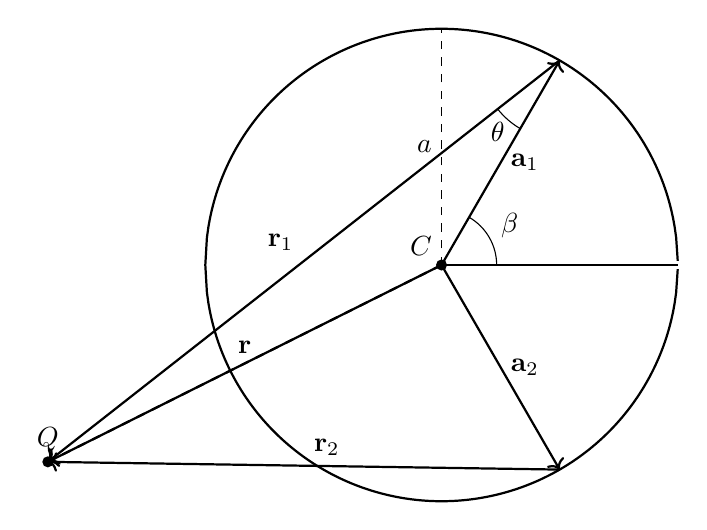
\begin{tikzpicture}
			
			
			\coordinate (A) at (0,0);
			\coordinate (B) at (-5,-2.5);
			\coordinate (C) at (1.5,2.598076211);
			\coordinate (D) at (1.5,-2.598076211);
			\coordinate (E) at (3,0);
	
			
			\draw[thick, domain=-3:3, samples=300] plot(\x, {sqrt(9-pow(\x,2))});
			\draw[thick, domain=-3:3, samples=300] plot(\x, {-sqrt(9-pow(\x,2))});
			
			\draw[thick,dashed, domain=-5:0, samples=300] plot(\x,{0.5*\x});
			\draw[dashed] (A) -- (0,3) node[midway,left]{$a$};
			\draw[->, thick] (C) -- (B) node[midway,above left]{$\textbf{r}_1$};
			\draw[->, thick] (D) -- (B) node[midway, above right]{$\textbf{r}_2$};
			\draw[->,thick] (A)--(B) node[midway, above]{$\textbf{r}$};
			
			\draw[->, thick] (A)--(C) node[midway, right] {$\textbf{a}_1$};
			
			\draw[->, thick] (A)--(D) node[midway, right] {$\textbf{a}_2$};
			
			\draw (A)--(E) ;
			
			\fill (A) circle (2pt) node[above left]{$C$};
			\fill (B) circle (2pt) node[above]{$Q$};
			
			\tkzMarkAngle(B,C,A);
			\tkzLabelAngle[pos=1.2](B,C,A){$\theta$};
			
			\tkzMarkAngle[size=0.7](E,A,C);
			\tkzLabelAngle[pos=1](E,A,C){$\beta$};
			
			
		\end{tikzpicture}
	\end{figure}
	
	A força $d\textbf{F}_1$ é então:
	
	\[
	d\textbf{F}_1=k\frac{Qdq}{r'^3}\textbf{r}_1
	\]
	
	Escrevendo $\textbf{r}_1$ em termos de $\textbf{i}$, $\textbf{j}$ e $\textbf{k}$:
	
	\[
	\textbf{r}_1=\textbf{r}-\textbf{a}_1
	\]
	
	\[
	\textbf{r}_1=-a\cos\beta\textbf{i}-a\sin\beta\textbf{j}+r\textbf{k}
	\]
	
	Definindo uma distribuição de carga uniforme $\lambda$ na parte superior:
	
	\[
	\lambda=\frac{dq}{d\beta a}\Rightarrow dq=\lambda d\beta a
	\]
	
	Ou seja:
	
	\[
	d\textbf{F}_1=k\frac{Q\lambda d\beta a}{r'^3}\left(-a\cos\beta\textbf{i}-a\sin\beta\textbf{j}+r\textbf{k}\right)
	\]
	
	\[
	\textbf{F}_1=k\frac{Q\lambda a}{r'^3}\int_{0}^{\pi}d\beta\left(-a\cos\beta\textbf{i}-a\sin\beta\textbf{j}+r\textbf{k}\right)
	\]
	
	\[
	\textbf{F}_1=k\frac{Q\lambda a}{r'^3}\left[\int_{0}^{\pi}-a\cos\beta d\beta\textbf{i}+\int_{0}^{\pi}-a\sin\beta d\beta\textbf{j}+\int_{0}^{\pi}rd\beta\textbf{k}\right]
	\]
	
	
	\[
	\textbf{F}_1=k\frac{Q\lambda a}{r'^3}\left[\cancelto{0}{-a\sin\beta\left.\right|_{0}^\pi\textbf{i}}-a(-\cos\beta\left.\right|_{0}^\pi)\textbf{j}+\beta\left.\right|_{0}^\pi r\textbf{k}\right]
	\]
	
	\[
	\textbf{F}_1=k\frac{Q\lambda a}{r'^3}\left[-2a\textbf{j}+r\pi\textbf{k}\right]
	\]
	
	A força $d\textbf{F}_2$ é:
	
	\[
	d\textbf{F}_2=-k\frac{Qdq}{r'^3}\textbf{r}_2
	\]
	
	Escrevendo $\textbf{r}_2$ em termos de $\textbf{i}$, $\textbf{j}$ e $\textbf{k}$:
	
	\[
	\textbf{r}_2=\textbf{r}-\textbf{a}_2
	\]
	
	\[
	\textbf{r}_2=r\textbf{k}-a(\cos\phi\textbf{i}+\sin\phi\textbf{j})
	\]
	
	\[
	\textbf{r}_2=-a\cos\phi\textbf{i}-a\sin\phi\textbf{j}+r\textbf{k}
	\]
	
	A distribuição de carga na parte inferior seria:
	
	\[
	\lambda=\frac{dq}{d\phi a}\Rightarrow dq=\lambda d\phi a
	\]
	
	Ou seja,
	
	\[
	d\textbf{F}_2=-k\frac{Q\lambda d\phi a}{r'^3}\left[-a\cos\phi\textbf{i}-a\sin\phi\textbf{j}+r\textbf{k}\right]
	\]
	
	\[
	\textbf{F}_2=-k\frac{Q\lambda a}{r'^3}\left[-a\textbf{i}\int_{\pi}^{2\pi}\cos\phi d\phi-a\textbf{j}\int_{\pi}^{2\pi}\sin\phi d\phi+r\textbf{k}\int_{\pi}^{2\pi}d\phi\right]
	\]
	
	\[
	\textbf{F}_2=-k\frac{Q\lambda a}{r'^3}\left[-a\textbf{i}\left(\sin\phi\left.\right|_{\pi}^{2\pi}\right)-a\textbf{j}\left(-\cos\phi\left.\right|_{\pi}^{2\pi}\right)+r\textbf{k}\left(\phi\left.\right|_{\pi}^{2\pi}\right)\right]
	\]
	
	\[
	\textbf{F}_2=-k\frac{Q\lambda a}{r'^3}\left[2a\textbf{j}+r\pi\textbf{k}\right]
	\]
	
	A força resultante será então de:
	
	\[
	\textbf{F}=\textbf{F}_1+\textbf{F}_2=k\frac{Q\lambda a}{r'^3}\left[-2a\textbf{j}+r\pi\textbf{k}\right]-k\frac{Q\lambda a}{r'^3}\left[2a\textbf{j}+r\pi\textbf{k}\right]
	\]
	
	\[
	\textbf{F}=k\frac{Q\lambda a}{r'^3}\left[-2a\textbf{j}+r\pi\textbf{k}-2a\textbf{j}-r\pi\textbf{k}\right]
	\]
	
	\[
	\textbf{F}=-k\frac{4Q\lambda a^2}{r'^3}\textbf{j}
	\]
	
	
	Por o sistema ser um cone temos que:
	
	\[
	r'^2=r^2+a^2\Rightarrow r'=\sqrt{r^2+a^2}\Rightarrow r'^3=(r^2+a^2)^{3/2}
	\]
	
	Além disso:
	
	\[
	\lambda=\frac{q_t}{2\pi a}
	\]
	
	Sendo $q_t$ a carga total que pode ser escrita como a diferença das cargas superior e inferior: $q_1-q_2$
	Ou seja:
	
	\[
	\textbf{F}=-k\frac{4Q(q_1-q_2) a^2}{2\pi a(r^2+a^2)^{3/2}}\textbf{j}
	\]
	
	\[
	\textbf{F}=-k\frac{2Q(q_1-q_2) a}{\pi(r^2+a^2)^{3/2}}\textbf{j}
	\]
	
	\[
	\textbf{F}=-\frac{Q(q_1-q_2) a}{2\epsilon_0\pi^2(r^2+a^2)^{3/2}}\textbf{j}
	\]
	
	Ou seja:
	
	\[
	\textbf{E}=-\frac{(q_1-q_2) a}{2\epsilon_0\pi^2(r^2+a^2)^{3/2}}\textbf{j}
	\]
	
	\end{document}